\documentclass{msuposter}
\usepackage{lipsum}
\usepackage{multirow}
\usepackage{tikz,wrapfig}
\usepackage{tikz}
\usetikzlibrary{decorations.pathreplacing}
\usetikzlibrary{arrows}
\newcommand{\mR}{\mathbb{R}}
\newcommand{\mN}{\mathbb{N}}
\newcommand{\cT}{\mathcal{T}}
\newcommand{\uh}{u_h}
\newcommand{\qh}{q_h}
\newcommand{\ph}{p_h}
\newcommand{\qhat}{\hat{q}}
\newcommand{\uhat}{\hat{u}}
\newcommand{\cB}{\mathcal{B}}
\newcommand{\cL}{\mathcal{L}}
\newcommand{\cO}{\mathcal{O}}
\newcommand{\euhat}{\hat{e}_{\uh}}
\newcommand{\eqhat}{\hat{e}_{\qh}}
\newcommand{\cP}{\mathcal{P}}
\newcommand{\projh}{\mathcal{S}}
\newcommand{\eu}{e_u}
\newcommand{\ep}{e_p}
\newcommand{\eq}{e_q}
\newcommand{\xiu}{\xi_u}
\newcommand{\xip}{\xi_p}
\newcommand{\xiq}{\xi_q}
\newcommand{\xiuhat}{\hat{\xi}_u}
\newcommand{\xiqhat}{\hat{\xi}_q}
%\theoremstyle{definition}
%\newtheorem{definition}{Definition}[section]
%\newtheorem{example}{Example}[section]
%\theoremstyle{plain}
%\newtheorem{theorem}{Theorem}[section]
%\newtheorem{corollary}{Corollary}[theorem]
%\newtheorem{lemma}[theorem]{Lemma}
%\newtheorem{proposition}[theorem]{Proposition}
\title{A Deep Learning Based  Discontinuous Galerkin Method for Hyperbolic Equations with Discontinuous Solutions and Random Uncertainties}
\author{\href{http://lylyu.com/}{\textbf{Liyao Lyu}} }
\institute{
Department of Computational Mathematics, Science and Engineering, Michigan State University,
lyuliyao@msu.edu\\
}

\newcommand{\colwidth}{0.3\linewidth}

\begin{document}
\begin{frame}{}
\begin{columns}[t]
\begin{column}{\colwidth}
\begin{block}{Abstract}
\large{We propose a deep learning based discontinuous Galerkin method (D2GM) to solve hyperbolic equations with discontinuous solutions and random uncertainties. The main computational challenges for such problems include discontinuities of the solutions and the curse of dimensionality due to uncertainties. Deep learning techniques have been favored for
high-dimensional problems but face difficulties when the solution is not smooth, thus have so far been mainly used for
viscous hyperbolic system that admits only smooth solutions.  We alleviate this difficulty by setting up the loss function using discrete shock capturing schemes--the discontinous Galerkin method as an example--since the solutions are smooth in the discrete space.  The convergence of D2GM is established via the Lax equivalence theorem kind of argument. The high-dimensional random space
is handled by the Monte-Carlo method. Such a setup makes the D2GM approximate high-dimensional functions over the random space with satisfactory accuracy at reasonable cost. The D2GM is found numerically to be first-order and second-order accurate for (stochastic) linear conservation law with smooth solutions using piecewise constant and piecewise linear basis functions, respectively. Numerous examples are given to verify the efficiency and the robustness of D2GM with the dimensionality of random variables up to $200$ for (stochastic) linear conservation law and (stochastic) Burgers' equation.}\end{block}


\begin{exampleblock}{Linear conservation law (Deterministic)}
\large
Consider 
 \begin{equation}\label{eqn:linear}
 \left\{
 \begin{aligned}
 	 &2d\pi u_t - \sum_{i=1}^d u_{x_i} = 0 & x\in [0,1]^d\\
 	 &u(0,x) = h(x) = \sin( 2 \pi \sum_{k=1}^d x^k)
 \end{aligned}\right.
 \end{equation}
 with periodic boundary condition, and the exact solution  $u(t,x) = \sin(t + 2 \pi \sum_{k=1}^d x^k)$, $d = 1,2,3$.
\begin{figure}
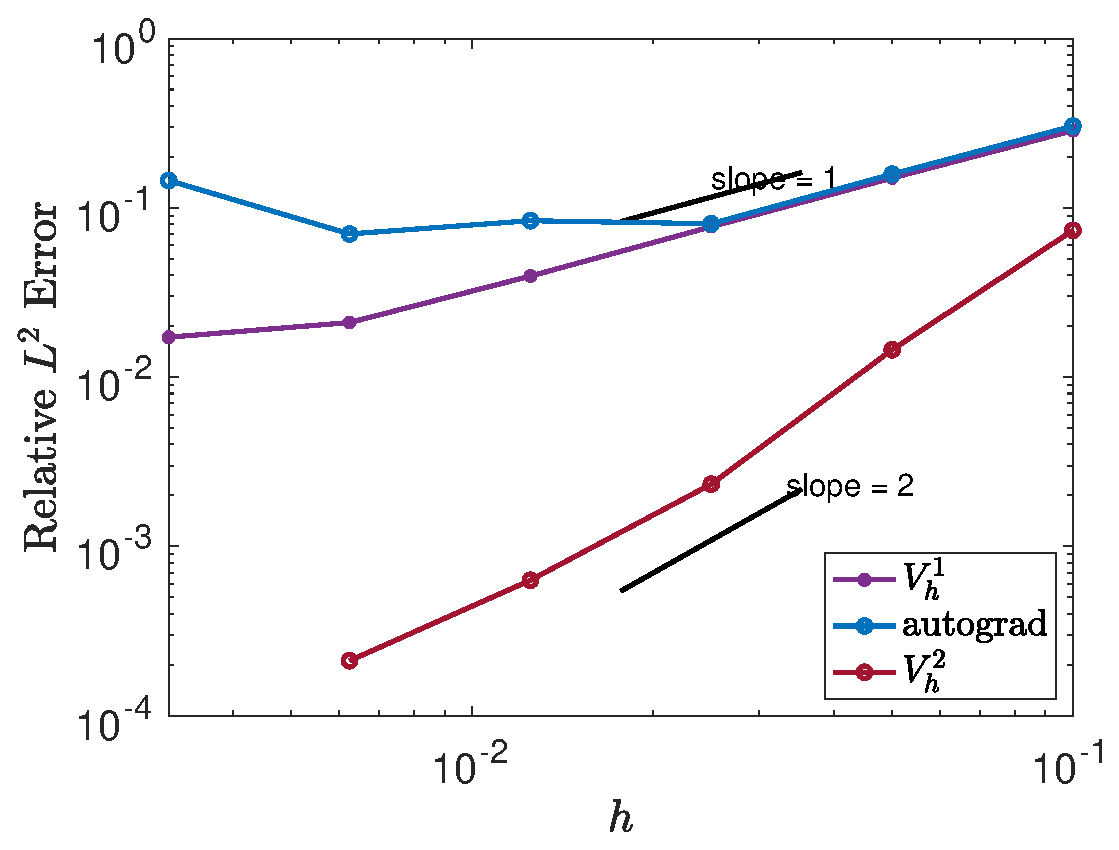
\includegraphics[width = 0.8 \linewidth]{Figure_linear_cv.eps}
\end{figure}
\end{exampleblock}
\end{column}



\begin{column}{\colwidth}
\begin{block}{Discontinuous element basis}

\begin{figure}[ht]
\centering
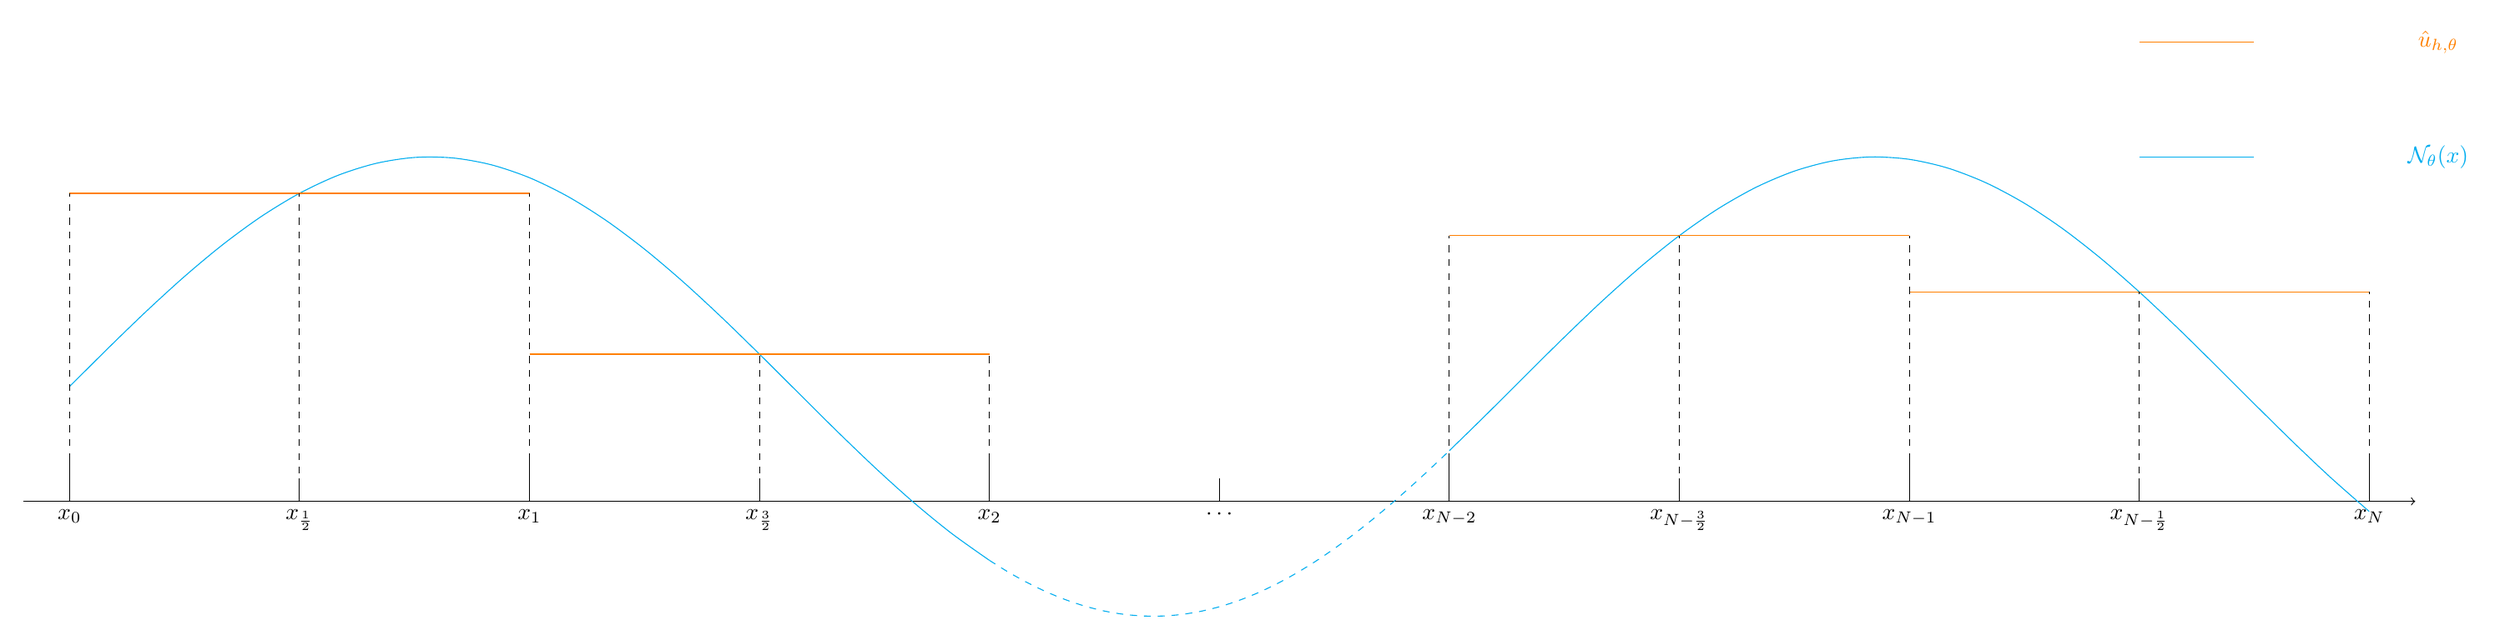
\begin{tikzpicture}[scale = 3.5]

	\draw[->] (-0.2,0)->(10.2,0);
	%画刻度
\foreach \x in {0,2,...,10}
{
    \draw[xshift=\x cm] (0,0) -- (0,0.2);
}; 
\foreach \x in {1,3,...,9}
{
    \draw[xshift=\x cm] (0,0) -- (0,0.1);
};  
%标x轴刻度值

\node[below] at(0,0){$x_0$};
\node[below] at(1,0){$x_{\frac{1}{2}}$};
\node[below] at(2,0){$x_1$};
\node[below] at(3,0){$x_\frac{3}{2}$};
\node[below] at(4,0){$x_2$};
\node[below] at(5,0){$\cdots$};
\node[below] at(6,0){$x_{N-2}$};
\node[below] at(7,0){$x_{N-\frac{3}{2}}$};
\node[below] at(8,0){$x_{N-1}$};
\node[below] at(9,0){$x_{N-\frac{1}{2}}$};
\node[below] (a) at(10,0){$x_N$};
\draw[cyan,domain=0:4,smooth] plot(\x,{sin(\x r)+0.5});
\draw[cyan,domain=6:10,smooth] plot(\x,{sin(\x r)+0.5});
\draw[cyan,domain=4:6,dashed,smooth] plot(\x,{sin(\x r)+0.5});
\draw[cyan,xshift = 10 cm, yshift = 1.5 cm] (-1,0) -- (-0.5,0) node at (0.3,0){$\mathcal{N}_\theta(x)$ };
\draw[orange,xshift = 10 cm, yshift = 2 cm] (-1,0) -- (-0.5,0) node at (0.3,0){$\hat{u}_{h,\theta}$ };
\foreach \x in {1,3}
{
\draw[orange,xshift = \x cm] (-1,{sin(\x r)+0.5}) -- (1,{sin(\x r)+0.5});
\draw[xshift = \x cm,dashed] (0,0) -- (0,{sin(\x r)+0.5});
\draw[xshift = \x cm,dashed] (-1,0) -- (-1,{sin(\x r)+0.5});
\draw[xshift = \x cm,dashed] (1,0) -- (1,{sin(\x r)+0.5});
}
\foreach \x in {7,9}
{
\draw[orange,xshift = \x cm] (-1,{sin(\x r)+0.5}) -- (1,{sin(\x r)+0.5});
\draw[xshift = \x cm,dashed] (0,0) -- (0,{sin(\x r)+0.5});
\draw[xshift = \x cm,dashed] (-1,0) -- (-1,{sin(\x r)+0.5});
\draw[xshift = \x cm,dashed] (1,0) -- (1,{sin(\x r)+0.5});
}

\end{tikzpicture}

\label{fig:element space}
\end{figure}
\large
\textcolor{orange}{$\hat{u}_{h,\theta}$ represents the numerical solution}\\
\textcolor{cyan}{$\mathcal{N}_\theta(x)$ represents the Neural Network}
\end{block}

\begin{exampleblock}{Burgers' equation (Deterministic)}
\large
Consider 
 \begin{equation}\label{eqn:bur}
 	u_t + (\frac{u^2}{2})_x = 0
 \end{equation} 
 with initial condition 
 \begin{equation}\label{eqn:bur ic}
 	u(0,x) = \left\{
 	\begin{matrix}
 		1 & x<0\\
 		 0 & x>0
 	\end{matrix}
 	\right.
 \end{equation}
 and reflect boundary condition
\begin{figure}
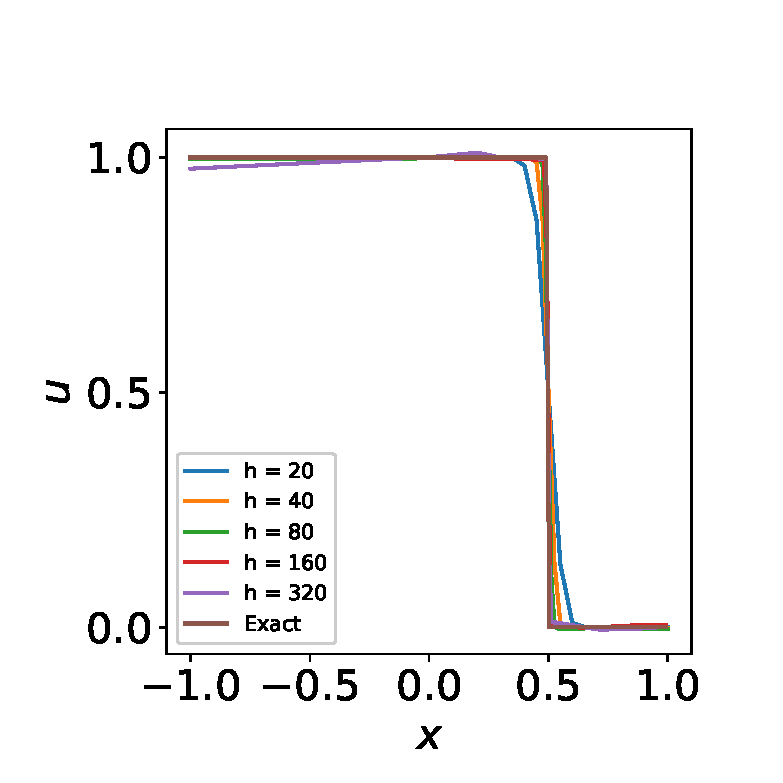
\includegraphics[width = 0.7\linewidth]{Burgus_equation_numerical_100.eps}
\end{figure}
\end{exampleblock}

\begin{exampleblock}{Linear conservation law (Stochastic)}
\large
Consider 
\begin{equation}\label{eqn:linear3Dstochastic}
	\begin{aligned}
		2 d  \pi u_t  - (1+\exp(-\sum_{j=1}^s \omega_j)^2) \sum_{i=1}^d u_{x_i}  = 0 
	\end{aligned}
\end{equation}
with periodic boundary condition and initial condition $u(0,\boldsymbol{x},\boldsymbol{\omega}) = \sin\left(2\pi \sum_{i=1}^d x_i \right) $. The exact solution of the problem is $u(t,\boldsymbol{x},\boldsymbol{\omega}) = \sin\left((1+\exp(-\sum_{j=1}^s \omega_j)^2) t + 2\pi \sum_{i=1}^d x_i\right)$.
\begin{table}[ht]
 \centering
 \begin{tabular}{|c|c|c|c|c|c|c|}
 \hline
     $s$ & $h = \Delta t$ &  Expectation & Order & Variance  & Order\\
 	\hline
     50 & 1/40 & 1.54 e-01 & & 2.13 e-01 &  \\
     50 & 1/80 & 7.85 e-02 & 0.97 & 1.14 e-01 & 0.93 \\
     50 & 1/160 & 3.88 e-02 & 1.01 & 5.61 e-02 & 0.96\\
     50 & 1/320 & 1.96 e-02 & 0.98 & 3.22 e-02 & 0.79\\
    \hline
	 100 & 1/40 & 1.53 e-01 &  & 2.07 e-01 & \\
	 100 & 1/80 & 7.83 e-02 & 0.97 &  1.12 e-01 & 0.88\\
	 100 & 1/160 & 3.93 e-02 & 0.99 & 5.82 e-02 & 0.95\\
	 100 & 1/320 & 2.01 e-02 & 0.96 &  2.93 e-02 & 0.98\\
\hline
 \end{tabular}
\label{tbl:cv error stochastic}	
\end{table}
\end{exampleblock}


\end{column}




\begin{column}{\colwidth}

\begin{exampleblock}{Burgers' equation (Stochastic)}
\large
Consider the stochastic Burgers' equation defined as
 \begin{equation}\label{eqn:bur stochastic}
 	u_t + (\frac{u^2}{2})_x = 0
 \end{equation} 
 with initial condition 
 \begin{equation}\label{eqn:bur stochastic ic}
 	u(0,x,\boldsymbol{\omega}) = \left\{
 	\begin{matrix}
 		1+\epsilon \sum_{i=1}^s \omega_i & x<0 \\
 		 0 & x>0 
 	\end{matrix}
 	\right..
 \end{equation}
The exact solution is
\begin{equation}
	 	u(t,x,\boldsymbol{\omega}) = \left\{
 	\begin{matrix}
 		z  & x< \frac{z}{2}\\
 		 0 & x>\frac{z}{2}
 	\end{matrix}
 	\right.,
\end{equation}
where $z = 1+\epsilon \sum_{i=1}^s \omega_i$. 
\begin{figure}
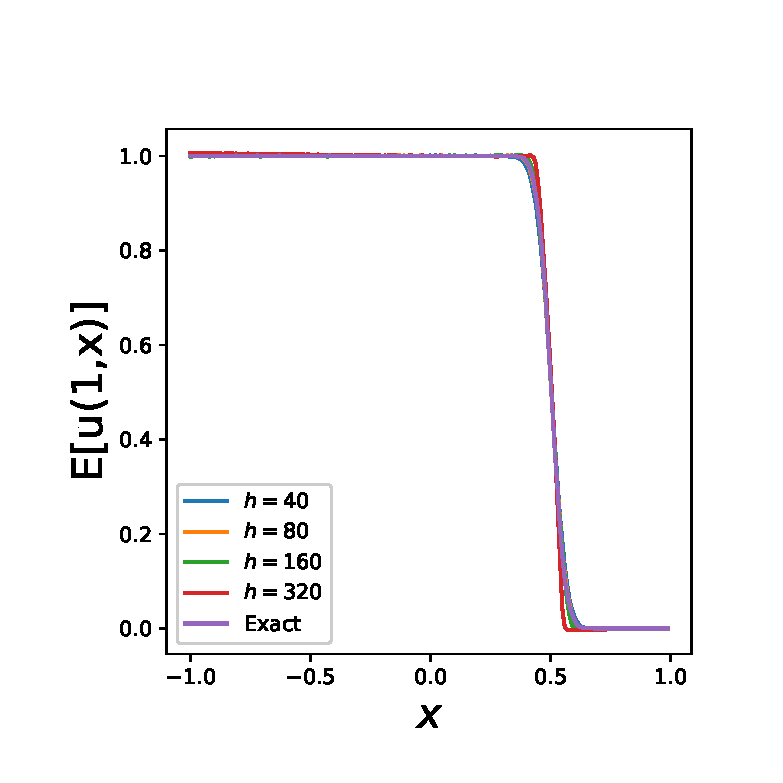
\includegraphics[width = 0.8\linewidth]{Burgus_equation_storchstic_dim_s_10_eps_005_E}
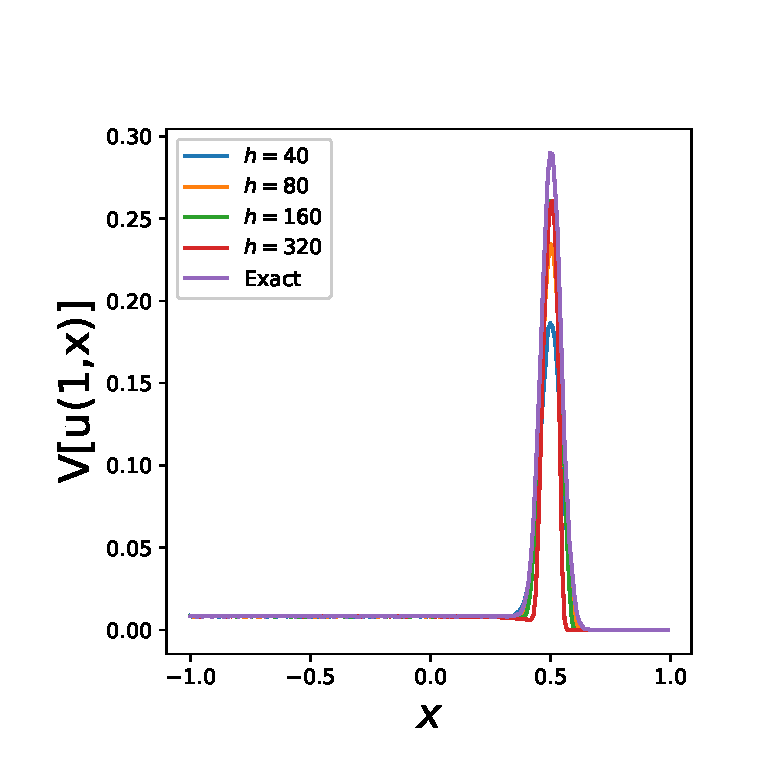
\includegraphics[width = 0.8\linewidth]{Burgus_equation_storchstic_dim_s_10_eps_005_V}
\end{figure}
\end{exampleblock}
\begin{block}{Reference}
Chen, Jingrun. Jin, Shi. Lyu, Liyao. 2021. "A Deep Learning Based Discontinuous Galerkin Method for Hyperbolic Equations with Discontinuous Solutions and Random Uncertainties."  arXiv 
\end{block}
\end{column}
\end{columns}	
\end{frame}
\end{document}
